%%% NUMBERING OF FIGURES %%%



\subsection{Methodological development and implementation}

It is known that similar proteins tend to bind similar ligands\cite{klabunde_chemogenomic_2007}, a principle behind many drug discovery projects\cite{sydow_advances_2019, keiser_relating_2007, falaguera_illuminating_2023}. We re-assessed the validity of this principle and found that, indeed, proteins from the same family (e.g. GPCRs) tend to have more similar active compounds than proteins from different families (Fig \ref{FigS1}). However, globally dissimilar proteins showing similar physicochemical and shape properties in their druggable pockets may still bind with similar ligands, which reasonably translates into a more precise and general form of the chemogenomics principle: similar pockets bind similar ligands\cite{gao_comprehensive_2013}. PocketVec builds on this observation to generate novel vector-type descriptors for characterizing protein small molecule binding pockets. 

Instead of directly characterizing the shape and physicochemical environment of the protein
cavities, we rely on a predefined set of small molecules and assess their potential binding to a
given pocket. More specifically, given a three-dimensional protein structure, we first identify
possible druggable pockets and we then use computational docking strategies to assess the
potential binding of the small molecules. The resulting docking scores are then translated into
rankings, which are finally stored in a vector-type format. In this way, each bit of the vector
represents the ranking of a predefined molecule, illustrating how good it binds with the pocket of
interest compared to all other molecules (Fig \ref{Fig1}). While the idea is conceptually pretty
straightforward, its implementation requires a thorough assessment of the set of used
molecules, the docking methodology and the benchmark strategy. The following sections
describe our effort to evaluate and optimize each step of the procedure.

%%%%%%%%%%%%%%%%
%%% FIGURE 1 %%%
%%%%%%%%%%%%%%%%

% \begin{figure}[htbp]
%   \centering
%   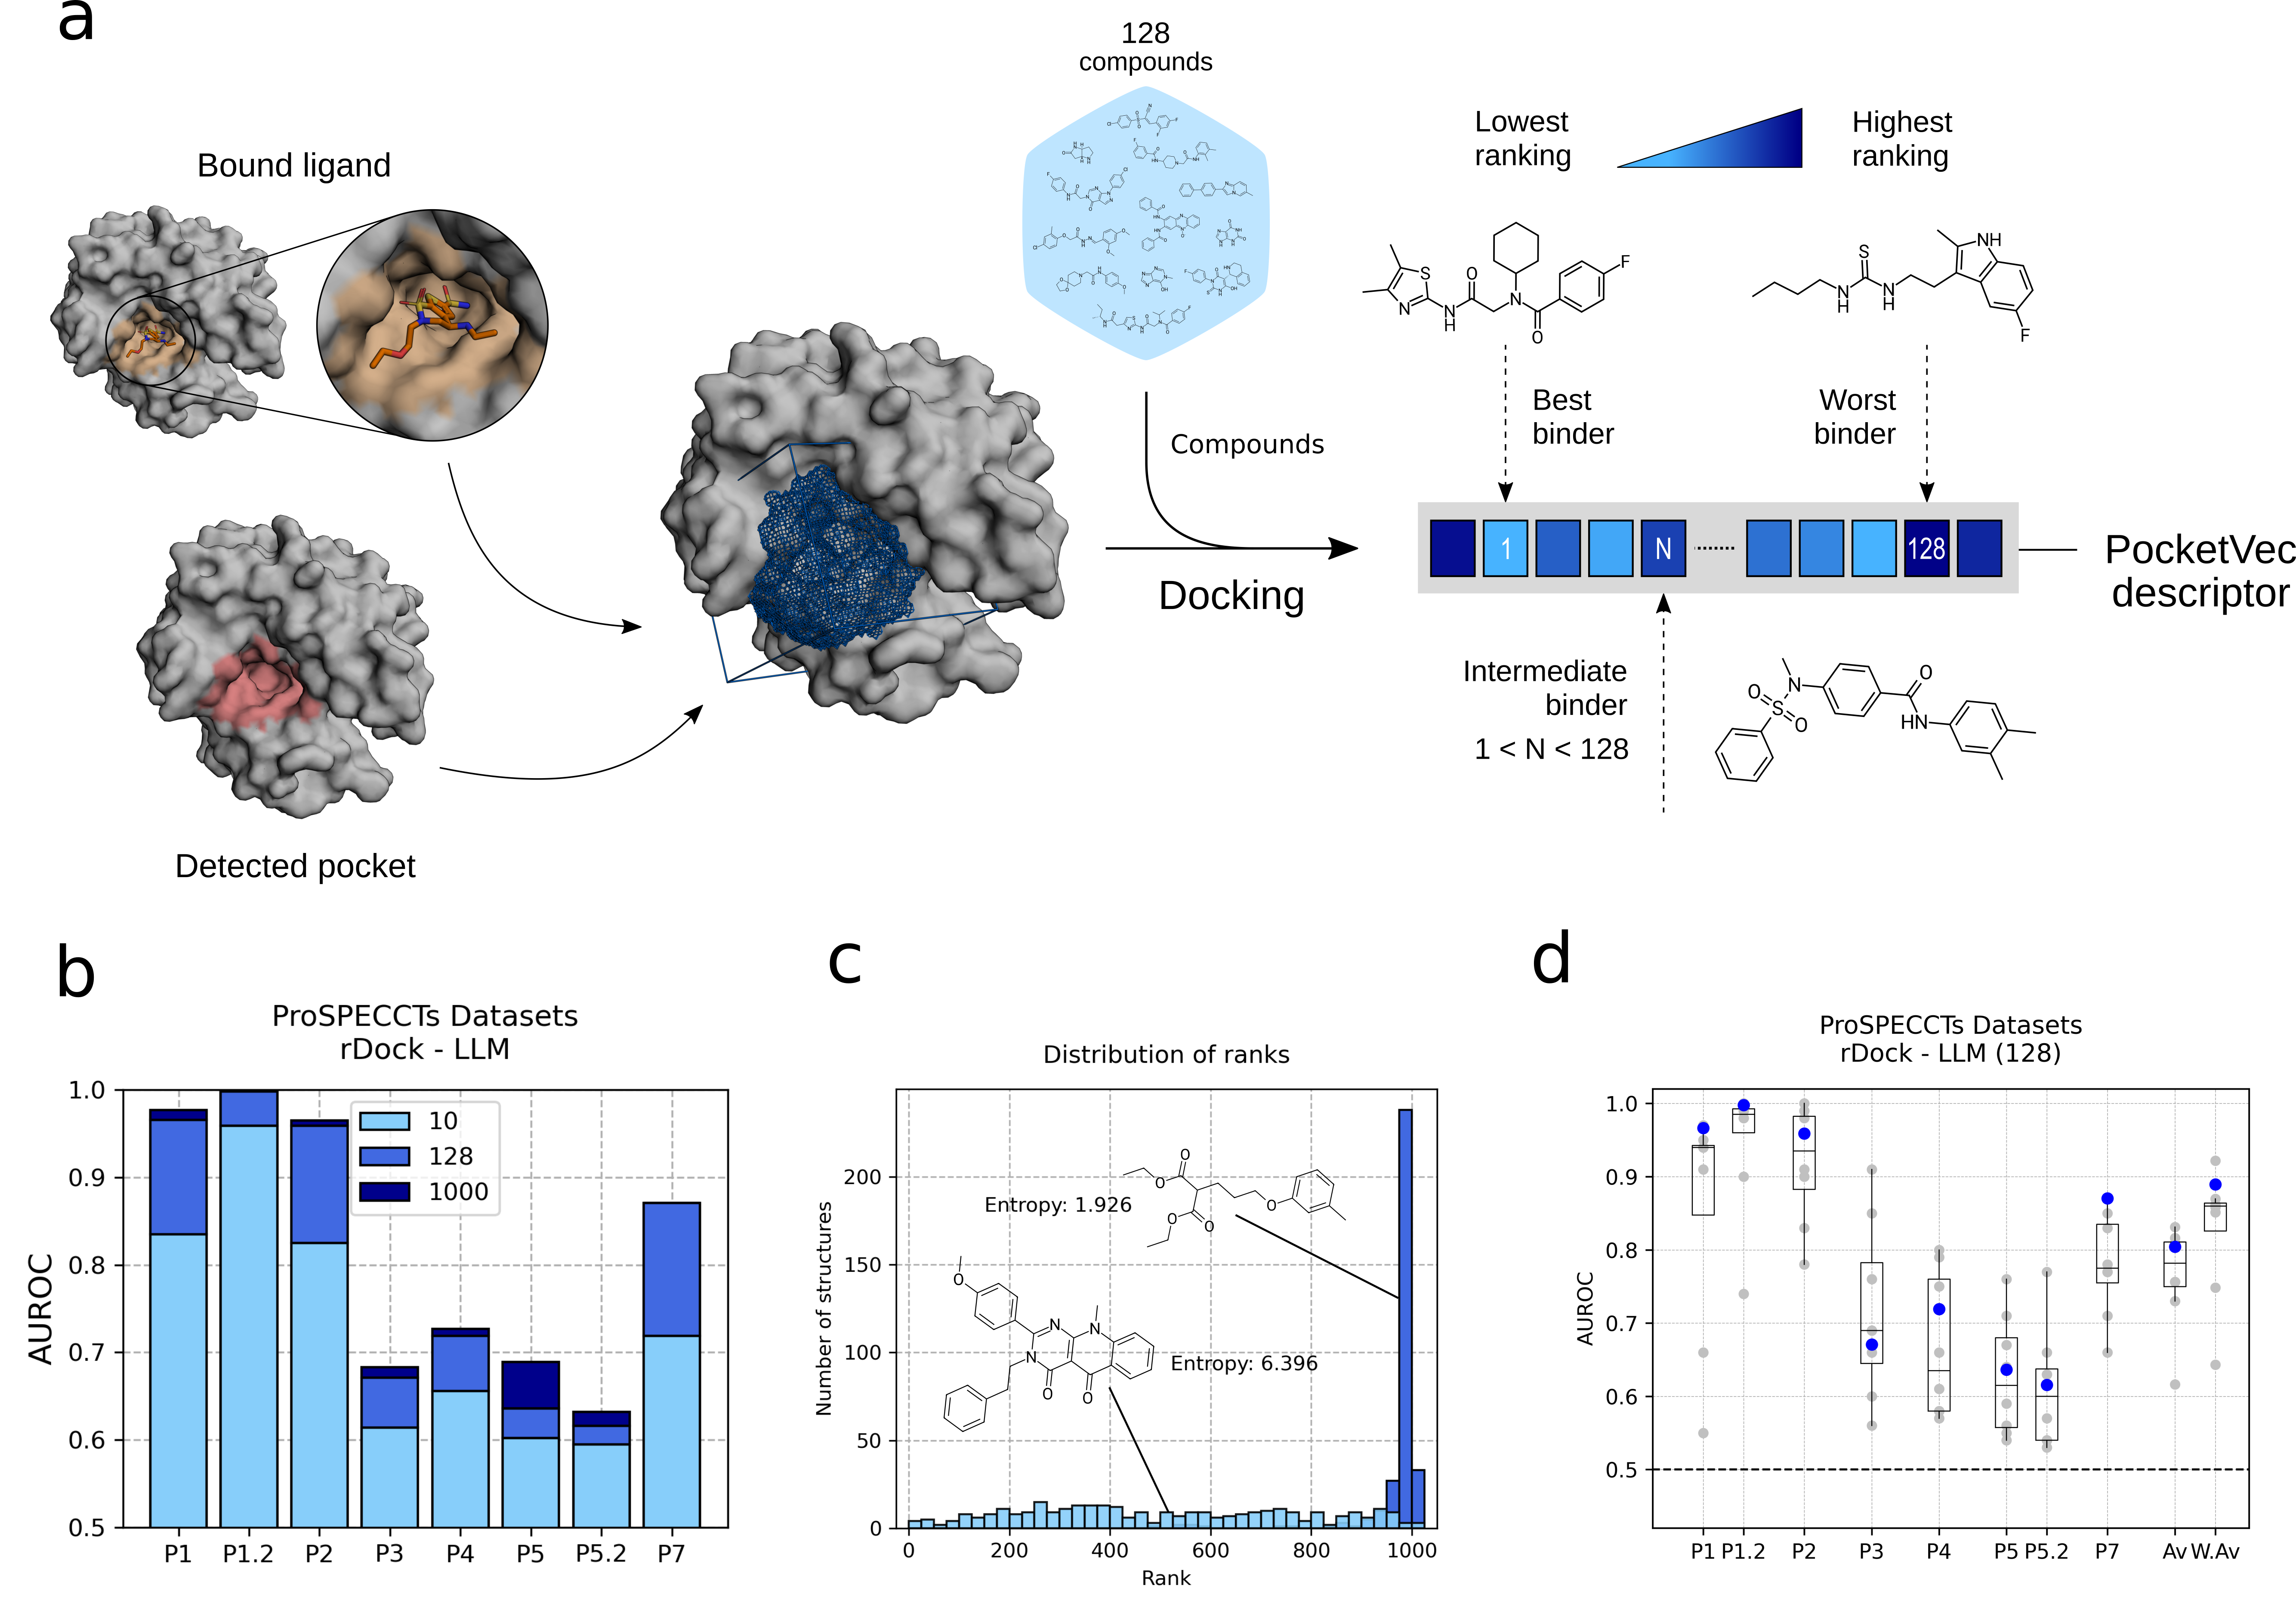
\includegraphics[width=\linewidth]{figures/PocketVec/Main/Fig1.png}
%   \caption{
%   Main title: PocketVec methodological pipeline and benchmark results. 
%   \begin{description}
%       \item[a] A
%       \item[b] A
%       \item[c] A
%       \item[d] A
%   \end{description}
%   }
%   \label{Fig1}
% \end{figure}

\begin{figure}[htbp]
  \centering
  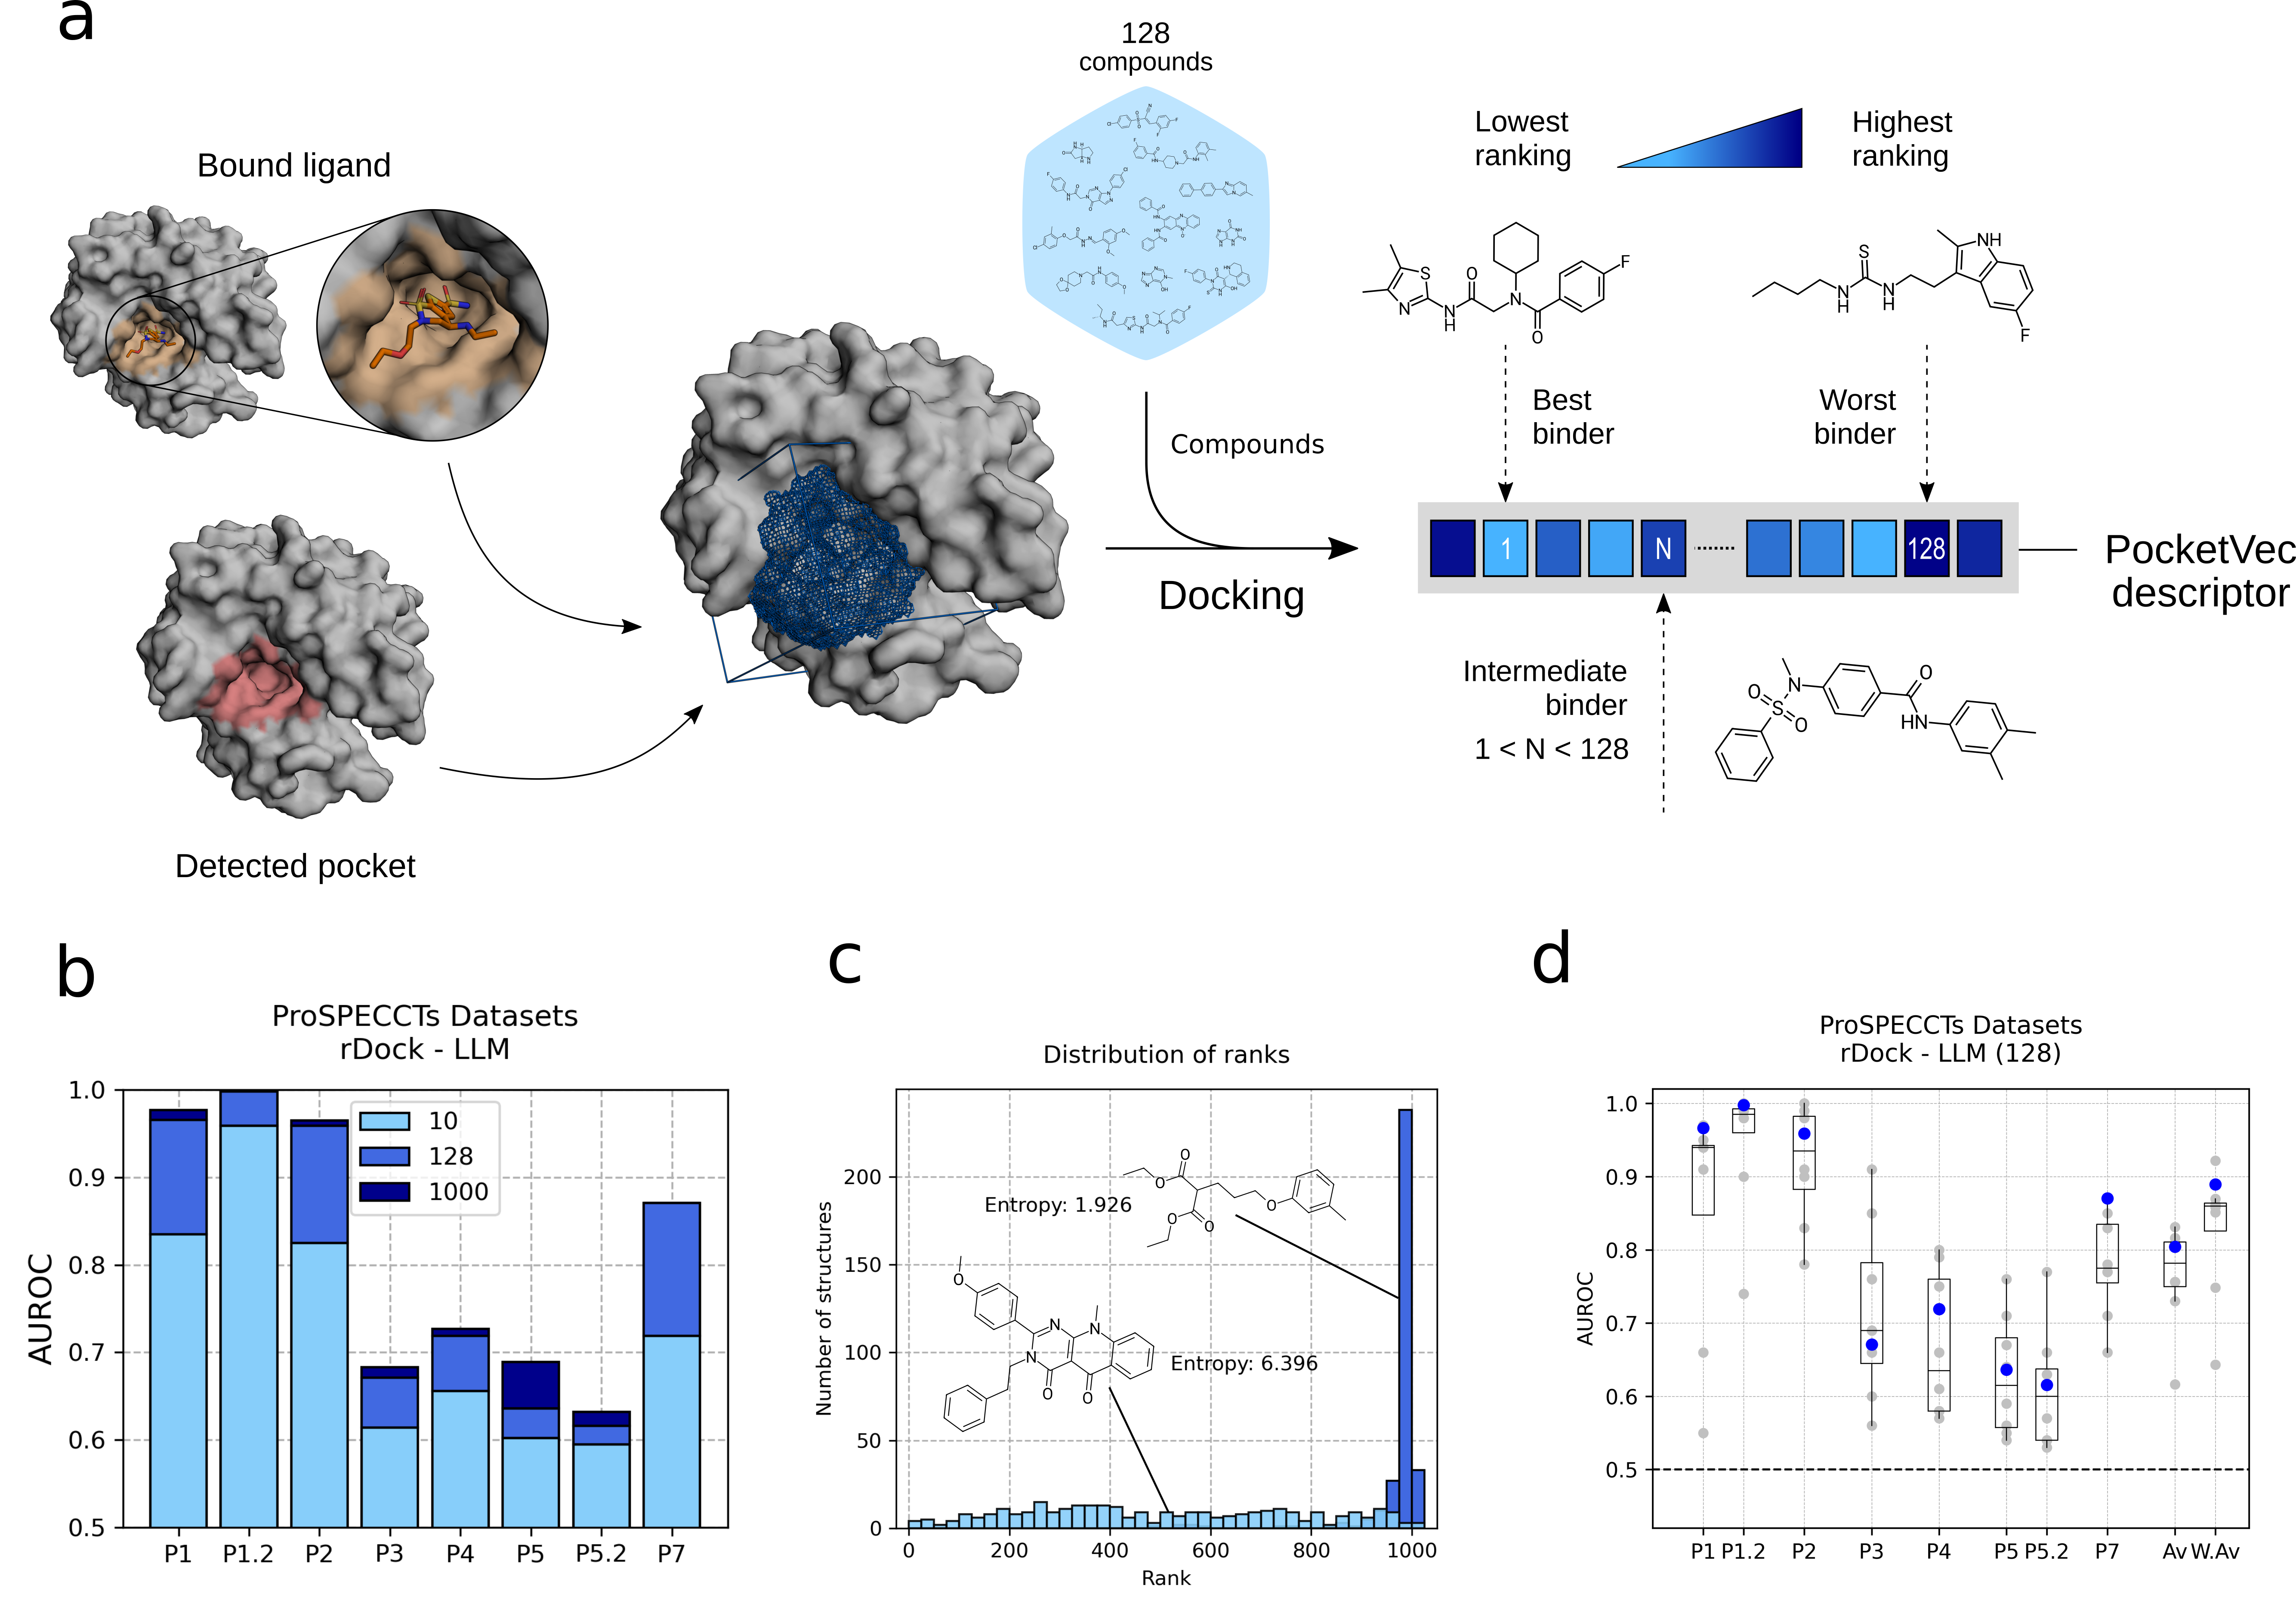
\includegraphics[width=\linewidth]{figures/PocketVec/Main/Fig1.png} 
  \caption{
    \textbf{PocketVec methodological pipeline and benchmark results.} 
    \textbf{a)} Given a 3D protein structure, binding site locations are established by the presence of bound ligands or by means of pocket detection algorithms. A predefined set of compounds (128 lead-like molecules in the standard PocketVec pipeline) is docked against the pocket of interest. The corresponding docking scores are then converted into rankings and stored in a vector-type format that serves to characterize the pocket. We refer to those vectors as PocketVec descriptors.
    \textbf{b)} Bars indicating the performance (AUROC, y-axis) of our descriptors generated with a varying number of predefined molecules among ProSPECCTs datasets (x-axis, P6 and P6.2 not included. For further details, please see Online Methods). Bar color indicates the number of predefined compounds (10, 128 and the complete set of 1,000 lead-like molecules, sorted by entropy). These results correspond to the rigid docking (rDock) and LLM combination. All the other combinations with all possible numbers of predefined compounds (from 1 to complete sets) are shown in Fig \ref{FigS7}.
    \textbf{c)} Predefined molecules with high and low entropy. The histograms depict the distribution (y-axis) of rankings (x-axis, bin width: 25) for the highest (sky blue) and lowest (dark blue) entropy lead-like molecules in ProSPECCTs P1. Their chemical structures are shown together with the corresponding entropy values.
    \textbf{d)} Performances (AUROC, y-axis) of distinct pocket descriptors among ProSPECCTs datasets (x-axis, P6 and P6.2 not included). Gray dots represent the individual performances of existing strategies to derive pocket descriptors (see Table \ref{TableS1}). Box plots indicate median (middle line), 25th, 75th percentile (box), and max and min value within the 1.5*25th and 1.5*75th percentile range (whiskers). Blue dots indicate the performance of PocketVec descriptors (128 LLM and rDock rigid docking). Av. values represent the average performance among ProSPECCTs datasets for each individual method and W. Av. values weight the average value according to the number of pairs within each dataset.
  }
  \label{Fig1}
\end{figure}